%!TeX root=../houndtop.tex
\chapter{Fixing the Nets}

\lettrine[ante=`,lines=4]{W}{e're} at close grips at last,' said Holmes as we walked together across the moor. »What a nerve the fellow has! How he pulled himself together in the face of what must have been a paralysing shock when he found that the wrong man had fallen a victim to his plot. I told you in London, Watson, and I tell you now again, that we have never had a foeman more worthy of our steel.«

»I am sorry that he has seen you.«

»And so was I at first. But there was no getting out of it.«

»What effect do you think it will have upon his plans now that he knows you are here?«

»It may cause him to be more cautious, or it may drive him to desperate measures at once. Like most clever criminals, he may be too confident in his own cleverness and imagine that he has completely deceived us.«

»Why should we not arrest him at once?«

»My dear Watson, you were born to be a man of action. Your instinct is always to do something energetic. But supposing, for argument's sake, that we had him arrested to-night, what on earth the better off should we be for that? We could prove nothing against him. There's the devilish cunning of it! If he were acting through a human agent we could get some evidence, but if we were to drag this great dog to the light of day it would not help us in putting a rope round the neck of its master.«

»Surely we have a case.«

»Not a shadow of one—only surmise and conjecture. We should be laughed out of court if we came with such a story and such evidence.«

»There is Sir Charles's death.«

»Found dead without a mark upon him. You and I know that he died of sheer fright, and we know also what frightened him; but how are we to get twelve stolid jurymen to know it? What signs are there of a hound? Where are the marks of its fangs? Of course we know that a hound does not bite a dead body and that Sir Charles was dead before ever the brute overtook him. But we have to prove all this, and we are not in a position to do it.«

»Well, then, to-night?«

»We are not much better off to-night. Again, there was no direct connection between the hound and the man's death. We never saw the hound. We heard it; but we could not prove that it was running upon this man's trail. There is a complete absence of motive. No, my dear fellow; we must reconcile ourselves to the fact that we have no case at present, and that it is worth our while to run any risk in order to establish one.«

»And how do you propose to do so?«

»I have great hopes of what Mrs Laura Lyons may do for us when the position of affairs is made clear to her. And I have my own plan as well. Sufficient for to-morrow is the evil thereof; but I hope before the day is past to have the upper hand at last.«

I could draw nothing further from him, and he walked, lost in thought, as far as the Baskerville gates.

»Are you coming up?«

»Yes; I see no reason for further concealment. But one last word, Watson. Say nothing of the hound to Sir Henry. Let him think that Selden's death was as Stapleton would have us believe. He will have a better nerve for the ordeal which he will have to undergo to-morrow, when he is engaged, if I remember your report aright, to dine with these people.«

»And so am I.«

»Then you must excuse yourself and he must go alone. That will be easily arranged. And now, if we are too late for dinner, I think that we are both ready for our suppers.«

Sir Henry was more pleased than surprised to see Sherlock Holmes, for he had for some days been expecting that recent events would bring him down from London. He did raise his eyebrows, however, when he found that my friend had neither any luggage nor any explanations for its absence. Between us we soon supplied his wants, and then over a belated supper we explained to the baronet as much of our experience as it seemed desirable that he should know. But first I had the unpleasant duty of breaking the news to Barrymore and his wife. To him it may have been an unmitigated relief, but she wept bitterly in her apron. To all the world he was the man of violence, half animal and half demon; but to her he always remained the little wilful boy of her own girlhood, the child who had clung to her hand. Evil indeed is the man who has not one woman to mourn him.

»I've been moping in the house all day since Watson went off in the morning,« said the baronet. »I guess I should have some credit, for I have kept my promise. If I hadn't sworn not to go about alone I might have had a more lively evening, for I had a message from Stapleton asking me over there.«

»I have no doubt that you would have had a more lively evening,« said Holmes drily. »By the way, I don't suppose you appreciate that we have been mourning over you as having broken your neck?«

Sir Henry opened his eyes. »How was that?«

»This poor wretch was dressed in your clothes. I fear your servant who gave them to him may get into trouble with the police.«

»That is unlikely. There was no mark on any of them, as far as I know.«

»That's lucky for him—in fact, it's lucky for all of you, since you are all on the wrong side of the law in this matter. I am not sure that as a conscientious detective my first duty is not to arrest the whole household. Watson's reports are most incriminating documents.«

»But how about the case?« asked the baronet. »Have you made anything out of the tangle? I don't know that Watson and I are much the wiser since we came down.«

»I think that I shall be in a position to make the situation rather more clear to you before long. It has been an exceedingly difficult and most complicated business. There are several points upon which we still want light—but it is coming all the same.«

»We've had one experience, as Watson has no doubt told you. We heard the hound on the moor, so I can swear that it is not all empty superstition. I had something to do with dogs when I was out West, and I know one when I hear one. If you can muzzle that one and put him on a chain I'll be ready to swear you are the greatest detective of all time.«

»I think I will muzzle him and chain him all right if you will give me your help.«

»Whatever you tell me to do I will do.«

»Very good; and I will ask you also to do it blindly, without always asking the reason.«

»Just as you like.«

»If you will do this I think the chances are that our little problem will soon be solved. I have no doubt\longdash«

He stopped suddenly and stared fixedly up over my head into the air. The lamp beat upon his face, and so intent was it and so still that it might have been that of a clear-cut classical statue, a personification of alertness and expectation.

\begin{figure}[tbph]
\centering
\includegraphics[width=\linewidth]{13_stopstare}
\caption{He stopped suddenly and stared fixedly}
\end{figure}

»What is it?« we both cried.

I could see as he looked down that he was repressing some internal emotion. His features were still composed, but his eyes shone with amused exultation.

»Excuse the admiration of a connoisseur,« said he as he waved his hand towards the line of portraits which covered the opposite wall. »Watson won't allow that I know anything of art, but that is mere jealousy, because our views upon the subject differ. Now, these are a really very fine series of portraits.«

»Well, I'm glad to hear you say so,« said Sir Henry, glancing with some surprise at my friend. »I don't pretend to know much about these things, and I'd be a better judge of a horse or a steer than of a picture. I didn't know that you found time for such things.«

%»I know what is good when I see it, and I see it now. That's a Kneller\footnote{Sir Godfrey Kneller (1646-1723) was the leading portraitist in England at the turn of the eighteenth century.}, I'll swear, that lady in the blue silk over yonder, and the stout gentleman with the wig ought to be a Reynolds\footnote{Sir Joshua Reynolds (1723-1792) was the leading portraitist in England in the later eighteenth century.}. They are all family portraits, I presume?«

»I know what is good when I see it, and I see it now. That's a Kneller, I'll swear, that lady in the blue silk over yonder, and the stout gentleman with the wig ought to be a Reynolds. They are all family portraits, I presume?«


»Every one.«

»Do you know the names?«

»Barrymore has been coaching me in them, and I think I can say my lessons fairly well.«

»Who is the gentleman with the telescope?«

%»That is Rear-Admiral Baskerville, who served under Rodney\footnote{Admiral George Brydges Rodney, 1st Baron Rodney, KB (1718-1792).} in the West Indies\footnote{Rodney's fleet saw a great deal of action in the Caribbean, including the invasion of Martinique (1762), part of the Seven Years' War; the capture of Sint Eustatius (1781), part of the Fourth Anglo-Dutch War; and the Battle of Saintes (1782), part of the American Revolutionary War.}. The man with the blue coat and the roll of paper is Sir William Baskerville, who was Chairman of Committees of the House of Commons under Pitt\footnote{William Pitt the Younger (1759-1806) was Prime Minister of Great Britain, then of the United Kingdom, between 1783 and 1806

»That is Rear-Admiral Baskerville, who served under Rodney in the West Indies. The man with the blue coat and the roll of paper is Sir William Baskerville, who was Chairman of Committees of the House of Commons under Pitt.«


»And this Cavalier opposite to me—the one with the black velvet and the lace?«

»Ah, you have a right to know about him. That is the cause of all the mischief, the wicked Hugo, who started the Hound of the Baskervilles. We're not likely to forget him.«

I gazed with interest and some surprise upon the portrait.

»Dear me!« said Holmes, »he seems a quiet, meek-mannered man enough, but I dare say that there was a lurking devil in his eyes. I had pictured him as a more robust and ruffianly person.«

»There's no doubt about the authenticity, for the name and the date, 1647, are on the back of the canvas.«

Holmes said little more, but the picture of the old roysterer seemed to have a fascination for him, and his eyes were continually fixed upon it during supper. It was not until later, when Sir Henry had gone to his room, that I was able to follow the trend of his thoughts. He led me back into the banqueting-hall, his bedroom candle in his hand, and he held it up against the time-stained portrait on the wall.

»Do you see anything there?«

I looked at the broad plumed hat, the curling love-locks, the white lace collar, and the straight, severe face which was framed between them. It was not a brutal countenance, but it was prim, hard, and stern, with a firm-set, thin-lipped mouth, and a coldly intolerant eye.

»Is it like anyone you know?«

»There is something of Sir Henry about the jaw.«

»Just a suggestion, perhaps. But wait an instant!« He stood upon a chair, and, holding up the light in his left hand, he curved his right arm over the broad hat and round the long ringlets.

»Good heavens!« I cried, in amazement.

The face of Stapleton had sprung out of the canvas.

»Ha, you see it now. My eyes have been trained to examine faces and not their trimmings. It is the first quality of a criminal investigator that he should see through a disguise.«

»But this is marvellous. It might be his portrait.«

»Yes, it is an interesting instance of a throwback, which appears to be both physical and spiritual. A study of family portraits is enough to convert a man to the doctrine of reincarnation. The fellow is a Baskerville—that is evident.«

»With designs upon the succession.«

\begin{figure}[tbh]
\centering
\includegraphics[width=.6\linewidth]{13_mirror}
\caption{»Good heavens!« I cried, in amazement.}
\end{figure}

»Exactly. This chance of the picture has supplied us with one of our most obvious missing links. We have him, Watson, we have him, and I dare swear that before to-morrow night he will be fluttering in our net as helpless as one of his own butterflies. A pin, a cork, and a card, and we add him to the Baker Street collection!« He burst into one of his rare fits of laughter as he turned away from the picture. I have not heard him laugh often, and it has always boded ill to somebody.

I was up betimes in the morning, but Holmes was afoot earlier still, for I saw him as I dressed, coming up the drive.

»Yes, we should have a full day to-day,« he remarked, and he rubbed his hands with the joy of action. »The nets are all in place, and the drag is about to begin. We'll know before the day is out whether we have caught our big, lean-jawed pike, or whether he has got through the meshes.«

»Have you been on the moor already?«

»I have sent a report from Grimpen to Princetown as to the death of Selden. I think I can promise that none of you will be troubled in the matter. And I have also communicated with my faithful Cartwright, who would certainly have pined away at the door of my hut, as a dog does at his master's grave, if I had not set his mind at rest about my safety.«

»What is the next move?«

»To see Sir Henry. Ah, here he is!«

»Good morning, Holmes,« said the baronet. »You look like a general who is planning a battle with his chief of the staff.«

»That is the exact situation. Watson was asking for orders.«

»And so do I.«

»Very good. You are engaged, as I understand, to dine with our friends the Stapletons to-night.«

»I hope that you will come also. They are very hospitable people, and I am sure that they would be very glad to see you.«

»I fear that Watson and I must go to London.«

»To London?«

»Yes, I think that we should be more useful there at the present juncture.«

The baronet's face perceptibly lengthened.

»I hoped that you were going to see me through this business. The Hall and the moor are not very pleasant places when one is alone.«

»My dear fellow, you must trust me implicitly and do exactly what I tell you. You can tell your friends that we should have been happy to have come with you, but that urgent business required us to be in town. We hope very soon to return to Devonshire. Will you remember to give them that message?«

»If you insist upon it.«

»There is no alternative, I assure you.«

I saw by the baronet's clouded brow that he was deeply hurt by what he regarded as our desertion.

»When do you desire to go?« he asked coldly.

»Immediately after breakfast. We will drive in to Coombe Tracey, but Watson will leave his things as a pledge that he will come back to you. Watson, you will send a note to Stapleton to tell him that you regret that you cannot come.«

»I have a good mind to go to London with you,« said the baronet. »Why should I stay here alone?«

»Because it is your post of duty. Because you gave me your word that you would do as you were told, and I tell you to stay.«

»All right, then, I'll stay.«

»One more direction! I wish you to drive to Merripit House. Send back your trap, however, and let them know that you intend to walk home.«

»To walk across the moor?«

»Yes.«

»But that is the very thing which you have so often cautioned me not to do.«

»This time you may do it with safety. If I had not every confidence in your nerve and courage I would not suggest it, but it is essential that you should do it.«

»Then I will do it.«

»And as you value your life do not go across the moor in any direction save along the straight path which leads from Merripit House to the Grimpen Road, and is your natural way home.«

»I will do just what you say.«

»Very good. I should be glad to get away as soon after breakfast as possible, so as to reach London in the afternoon.«

I was much astounded by this programme, though I re\-mem\-bered that Holmes had said to Stapleton on the night before that his visit would terminate next day. It had not crossed my mind, however, that he would wish me to go with him, nor could I understand how we could both be absent at a moment which he himself declared to be critical. There was nothing for it, however, but implicit obedience; so we bade good-bye to our rueful friend, and a couple of hours afterwards we were at the station of Coombe Tracey and had dispatched the trap upon its return journey. A small boy was waiting upon the platform.

»Any orders, sir?«

»You will take this train to town, Cartwright. The moment you arrive you will send a wire to Sir Henry Baskerville, in my name, to say that if he finds the pocket-book which I have dropped he is to send it by registered post to Baker Street.«

»Yes, sir.«

»And ask at the station office if there is a message for me.«

The boy returned with a telegram, which Holmes handed to me. It ran: 
\begin{samepage}
\blockquote{
\textsc{Wire received. Coming down with unsigned warrant. Arrive five-forty.}
\begin{flushright}
—  {\small\scshape LESTRADE.}
\end{flushright}
}
\end{samepage}

»That is in answer to mine of this morning. He is the best of the professionals, I think, and we may need his assistance. Now, Watson, I think that we cannot employ our time better than by calling upon your acquaintance, Mrs Laura Lyons.«

His plan of campaign was beginning to be evident. He would use the baronet in order to convince the Stapletons that we were really gone, while we should actually return at the instant when we were likely to be needed. That telegram from London, if mentioned by Sir Henry to the Stapletons, must remove the last suspicions from their minds. Already I seemed to see our nets drawing closer around that lean-jawed pike.

Mrs Laura Lyons was in her office, and Sherlock Holmes opened his interview with a frankness and directness which considerably amazed her.

»I am investigating the circumstances which attended the death of the late Sir Charles Baskerville,« said he. »My friend here, Dr Watson, has informed me of what you have communicated, and also of what you have withheld in connection with that matter.«

»What have I withheld?« she asked defiantly.

»You have confessed that you asked Sir Charles to be at the gate at ten o'clock. We know that that was the place and hour of his death. You have withheld what the connection is between these events.«

»There is no connection.«

»In that case the coincidence must indeed be an extraordinary one. But I think that we shall succeed in establishing a connection after all. I wish to be perfectly frank with you, Mrs Lyons. We regard this case as one of murder, and the evidence may implicate not only your friend Mr Stapleton, but his wife as well.«

\begin{figure}[tbh]
\centering
\includegraphics[width=.7\linewidth]{13_sprang}
\caption{The lady sprang from her chair}
\end{figure}
%\afterpage{\clearpage}

The lady sprang from her chair.

»His wife!« she cried.

»The fact is no longer a secret. The person who has passed for his sister is really his wife.«

Mrs Lyons had resumed her seat. Her hands were grasping the arms of her chair, and I saw that the pink nails had turned white with the pressure of her grip.

»His wife!« she said again. »His wife! He is not a married man.«

Sherlock Holmes shrugged his shoulders.

»Prove it to me! Prove it to me! And if you can do so— !« The fierce flash of her eyes said more than any words.

»I have come prepared to do so,« said Holmes, drawing several papers from his pocket. »Here is a photograph of the couple taken in York four years ago. It is indorsed »Mr and Mrs Vandeleur«, but you will have no difficulty in recognizing him, and her also, if you know her by sight. Here are three written descriptions by trustworthy witnesses of Mr and Mrs Vandeleur, who at that time kept St Oliver's private school. Read them and see if you can doubt the identity of these people.«

She glanced at them, and then looked up at us with the set, rigid face of a desperate woman.

»Mr Holmes,« she said, »this man had offered me marriage on condition that I could get a divorce from my husband. He has lied to me, the villain, in every conceivable way. Not one word of truth has he ever told me. And why—why? I imagined that all was for my own sake. But now I see that I was never anything but a tool in his hands. Why should I preserve faith with him who never kept any with me? Why should I try to shield him from the consequences of his own wicked acts? Ask me what you like, and there is nothing which I shall hold back. One thing I swear to you, and that is that when I wrote the letter I never dreamed of any harm to the old gentleman, who had been my kindest friend.«

»I entirely believe you, madam,« said Sherlock Holmes. »The recital of these events must be very painful to you, and perhaps it will make it easier if I tell you what occurred, and you can check me if I make any material mistake. The sending of this letter was suggested to you by Stapleton?«

»He dictated it.«

»I presume that the reason he gave was that you would receive help from Sir Charles for the legal expenses connected with your divorce?«

»Exactly.«

»And then after you had sent the letter he dissuaded you from keeping the appointment?«

»He told me that it would hurt his self-respect that any other man should find the money for such an object, and that though he was a poor man himself he would devote his last penny to removing the obstacles which divided us.«

»He appears to be a very consistent character. And then you heard nothing until you read the reports of the death in the paper?«

»No.«

»And he made you swear to say nothing about your appointment with Sir Charles?«

»He did. He said that the death was a very mysterious one, and that I should certainly be suspected if the facts came out. He frightened me into remaining silent.«

»Quite so. But you had your suspicions?«

She hesitated and looked down.

»I knew him,« she said. »But if he had kept faith with me I should always have done so with him.«

»I think that on the whole you have had a fortunate escape,« said Sherlock Holmes. »You have had him in your power and he knew it, and yet you are alive. You have been walking for some months very near to the edge of a precipice. We must wish you good-morning now, Mrs Lyons, and it is probable that you will very shortly hear from us again.«

»Our case becomes rounded off, and difficulty after difficulty thins away in front of us,« said Holmes as we stood waiting for the arrival of the express from town. »I shall soon be in the position of being able to put into a single connected narrative one of the most singular and sensational crimes of modern times. Students of criminology will remember the analogous incidents in Godno, in Little Russia, in the year `66, and of course there are the Anderson murders in North Carolina, but this case possesses some features which are entirely its own. Even now we have no clear case against this very wily man. But I shall be very much surprised if it is not clear enough before we go to bed this night.«

The London express came roaring into the station, and a small, wiry bulldog of a man had sprung from a first-class carriage. We all three shook hands, and I saw at once from the reverential way in which Lestrade gazed at my companion that he had learned a good deal since the days when they had first worked together. I could well remember the scorn which the theories of the reasoner used then to excite in the practical man.

\begin{figure}[p]
\centering
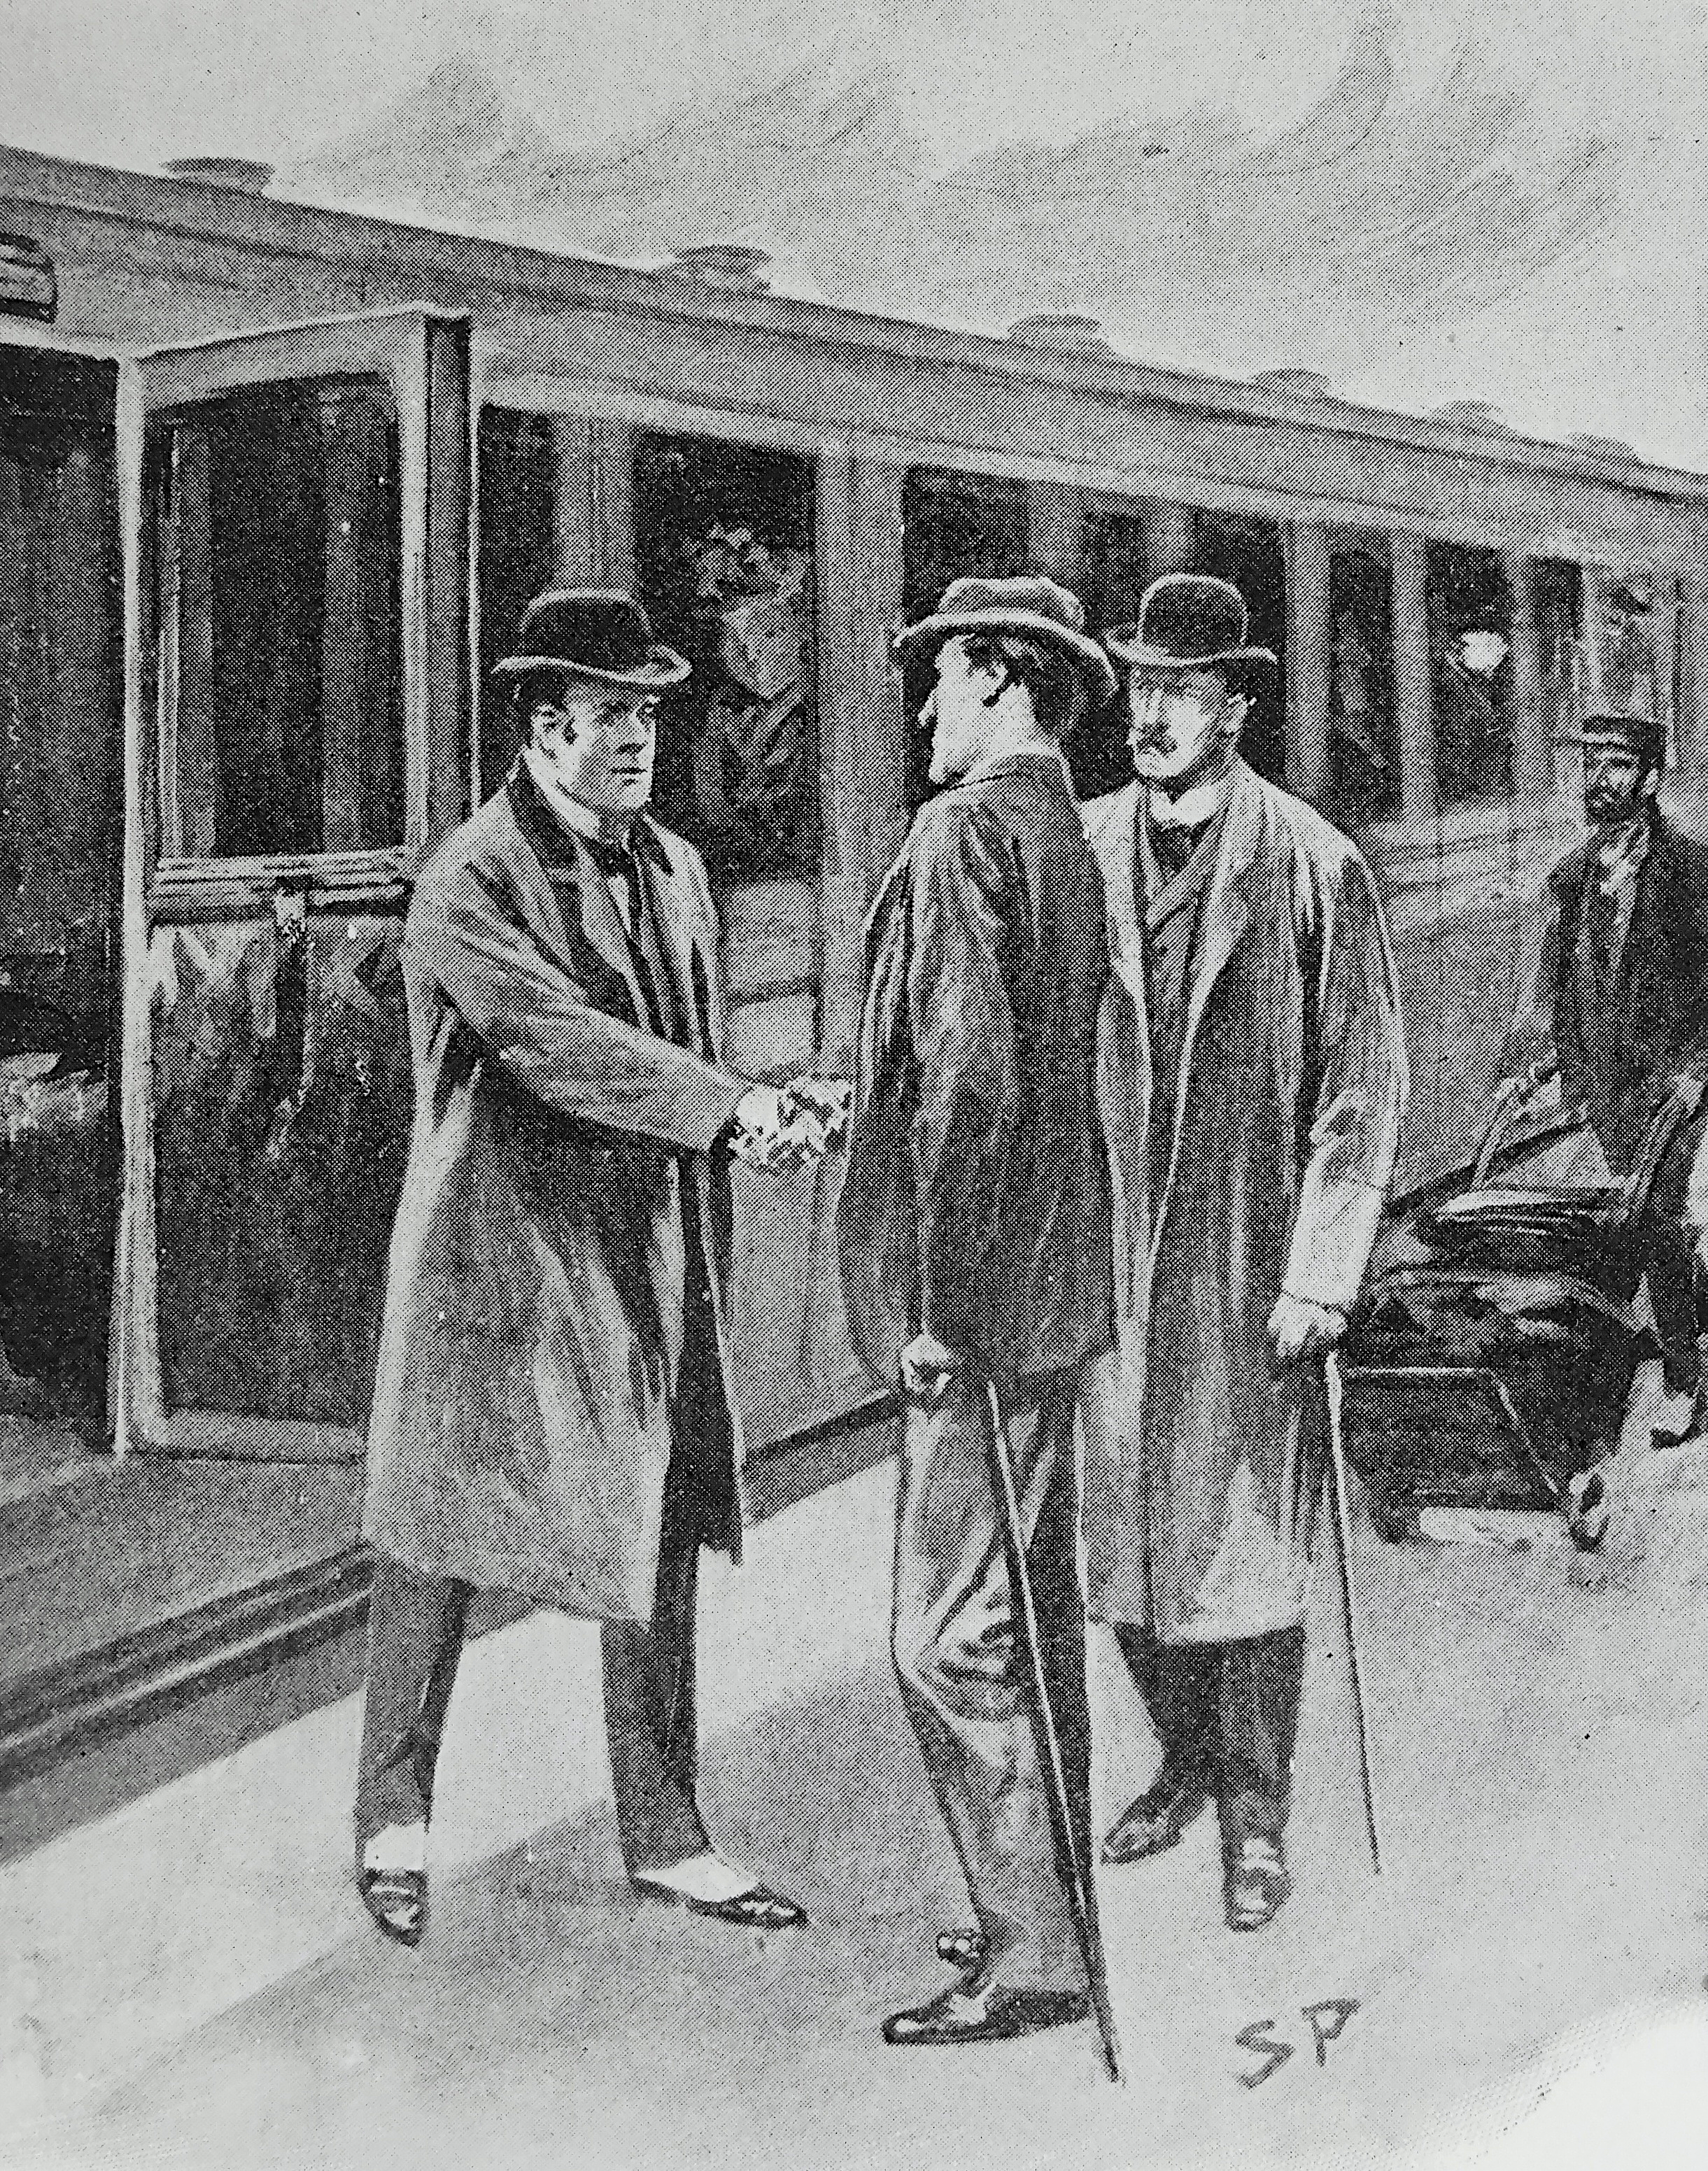
\includegraphics[width=\linewidth]{13_shookhands}
\caption{We all three shook hands}
\end{figure}

»Anything good?« he asked.

»The biggest thing for years,« said Holmes. »We have two hours before we need think of starting. I think we might employ it in getting some dinner and then, Lestrade, we will take the London fog out of your throat by giving you a breath of the pure night air of Dartmoor. Never been there? Ah, well, I don't suppose you will forget your first visit.«
%\cleardoubleevenpage
%\vfill
%\begin{figure}[tbph]
%\centering
%\includegraphics[width=\linewidth]{14_thehound}
%\caption{The Hound of the Baskervilles}
%\end{figure}
%\vfill
%\thispagestyle{empty}
%\clearpage